% Options for packages loaded elsewhere
\PassOptionsToPackage{unicode}{hyperref}
\PassOptionsToPackage{hyphens}{url}
\PassOptionsToPackage{dvipsnames,svgnames,x11names}{xcolor}
%
\documentclass[
  authoryear,
  3p]{elsarticle}

\usepackage{amsmath,amssymb}
\usepackage{iftex}
\ifPDFTeX
  \usepackage[T1]{fontenc}
  \usepackage[utf8]{inputenc}
  \usepackage{textcomp} % provide euro and other symbols
\else % if luatex or xetex
  \usepackage{unicode-math}
  \defaultfontfeatures{Scale=MatchLowercase}
  \defaultfontfeatures[\rmfamily]{Ligatures=TeX,Scale=1}
\fi
\usepackage{lmodern}
\ifPDFTeX\else  
    % xetex/luatex font selection
\fi
% Use upquote if available, for straight quotes in verbatim environments
\IfFileExists{upquote.sty}{\usepackage{upquote}}{}
\IfFileExists{microtype.sty}{% use microtype if available
  \usepackage[]{microtype}
  \UseMicrotypeSet[protrusion]{basicmath} % disable protrusion for tt fonts
}{}
\makeatletter
\@ifundefined{KOMAClassName}{% if non-KOMA class
  \IfFileExists{parskip.sty}{%
    \usepackage{parskip}
  }{% else
    \setlength{\parindent}{0pt}
    \setlength{\parskip}{6pt plus 2pt minus 1pt}}
}{% if KOMA class
  \KOMAoptions{parskip=half}}
\makeatother
\usepackage{xcolor}
\setlength{\emergencystretch}{3em} % prevent overfull lines
\setcounter{secnumdepth}{5}
% Make \paragraph and \subparagraph free-standing
\makeatletter
\ifx\paragraph\undefined\else
  \let\oldparagraph\paragraph
  \renewcommand{\paragraph}{
    \@ifstar
      \xxxParagraphStar
      \xxxParagraphNoStar
  }
  \newcommand{\xxxParagraphStar}[1]{\oldparagraph*{#1}\mbox{}}
  \newcommand{\xxxParagraphNoStar}[1]{\oldparagraph{#1}\mbox{}}
\fi
\ifx\subparagraph\undefined\else
  \let\oldsubparagraph\subparagraph
  \renewcommand{\subparagraph}{
    \@ifstar
      \xxxSubParagraphStar
      \xxxSubParagraphNoStar
  }
  \newcommand{\xxxSubParagraphStar}[1]{\oldsubparagraph*{#1}\mbox{}}
  \newcommand{\xxxSubParagraphNoStar}[1]{\oldsubparagraph{#1}\mbox{}}
\fi
\makeatother


\providecommand{\tightlist}{%
  \setlength{\itemsep}{0pt}\setlength{\parskip}{0pt}}\usepackage{longtable,booktabs,array}
\usepackage{calc} % for calculating minipage widths
% Correct order of tables after \paragraph or \subparagraph
\usepackage{etoolbox}
\makeatletter
\patchcmd\longtable{\par}{\if@noskipsec\mbox{}\fi\par}{}{}
\makeatother
% Allow footnotes in longtable head/foot
\IfFileExists{footnotehyper.sty}{\usepackage{footnotehyper}}{\usepackage{footnote}}
\makesavenoteenv{longtable}
\usepackage{graphicx}
\makeatletter
\def\maxwidth{\ifdim\Gin@nat@width>\linewidth\linewidth\else\Gin@nat@width\fi}
\def\maxheight{\ifdim\Gin@nat@height>\textheight\textheight\else\Gin@nat@height\fi}
\makeatother
% Scale images if necessary, so that they will not overflow the page
% margins by default, and it is still possible to overwrite the defaults
% using explicit options in \includegraphics[width, height, ...]{}
\setkeys{Gin}{width=\maxwidth,height=\maxheight,keepaspectratio}
% Set default figure placement to htbp
\makeatletter
\def\fps@figure{htbp}
\makeatother

\usepackage{booktabs}
\usepackage{longtable}
\usepackage{array}
\usepackage{multirow}
\usepackage{wrapfig}
\usepackage{float}
\usepackage{colortbl}
\usepackage{pdflscape}
\usepackage{tabu}
\usepackage{threeparttable}
\usepackage{threeparttablex}
\usepackage[normalem]{ulem}
\usepackage{makecell}
\usepackage{xcolor}
\makeatletter
\@ifpackageloaded{caption}{}{\usepackage{caption}}
\AtBeginDocument{%
\ifdefined\contentsname
  \renewcommand*\contentsname{Table of contents}
\else
  \newcommand\contentsname{Table of contents}
\fi
\ifdefined\listfigurename
  \renewcommand*\listfigurename{List of Figures}
\else
  \newcommand\listfigurename{List of Figures}
\fi
\ifdefined\listtablename
  \renewcommand*\listtablename{List of Tables}
\else
  \newcommand\listtablename{List of Tables}
\fi
\ifdefined\figurename
  \renewcommand*\figurename{Figure}
\else
  \newcommand\figurename{Figure}
\fi
\ifdefined\tablename
  \renewcommand*\tablename{Table}
\else
  \newcommand\tablename{Table}
\fi
}
\@ifpackageloaded{float}{}{\usepackage{float}}
\floatstyle{ruled}
\@ifundefined{c@chapter}{\newfloat{codelisting}{h}{lop}}{\newfloat{codelisting}{h}{lop}[chapter]}
\floatname{codelisting}{Listing}
\newcommand*\listoflistings{\listof{codelisting}{List of Listings}}
\makeatother
\makeatletter
\makeatother
\makeatletter
\@ifpackageloaded{caption}{}{\usepackage{caption}}
\@ifpackageloaded{subcaption}{}{\usepackage{subcaption}}
\makeatother
\journal{Journal of Economic Geography}

\ifLuaTeX
  \usepackage{selnolig}  % disable illegal ligatures
\fi
\usepackage[]{natbib}
\bibliographystyle{elsarticle-harv}
\usepackage{bookmark}

\IfFileExists{xurl.sty}{\usepackage{xurl}}{} % add URL line breaks if available
\urlstyle{same} % disable monospaced font for URLs
\hypersetup{
  pdftitle={A multi-scale story of the diffusion of a new technology: the Web},
  colorlinks=true,
  linkcolor={blue},
  filecolor={Maroon},
  citecolor={Blue},
  urlcolor={Blue},
  pdfcreator={LaTeX via pandoc}}


\setlength{\parindent}{6pt}
\begin{document}

\begin{frontmatter}
\title{A multi-scale story of the diffusion of a new technology: the
Web}


%\cortext[cor1]{Corresponding author}
        





\end{frontmatter}
    

\setcounter{section}{0}
\renewcommand{\thesection}{\Alph{section}}
\setcounter{table}{0}
\renewcommand{\thetable}{A\arabic{table}}
\setcounter{figure}{0}
\renewcommand{\thefigure}{A\arabic{figure}}
\setcounter{equation}{0}
\renewcommand{\theequation}{A\arabic{equation}}

\section{Appendix}\label{appendix}

\counterwithin{figure}{section}
\counterwithin{table}{section}

\begin{figure}[H]

{\centering 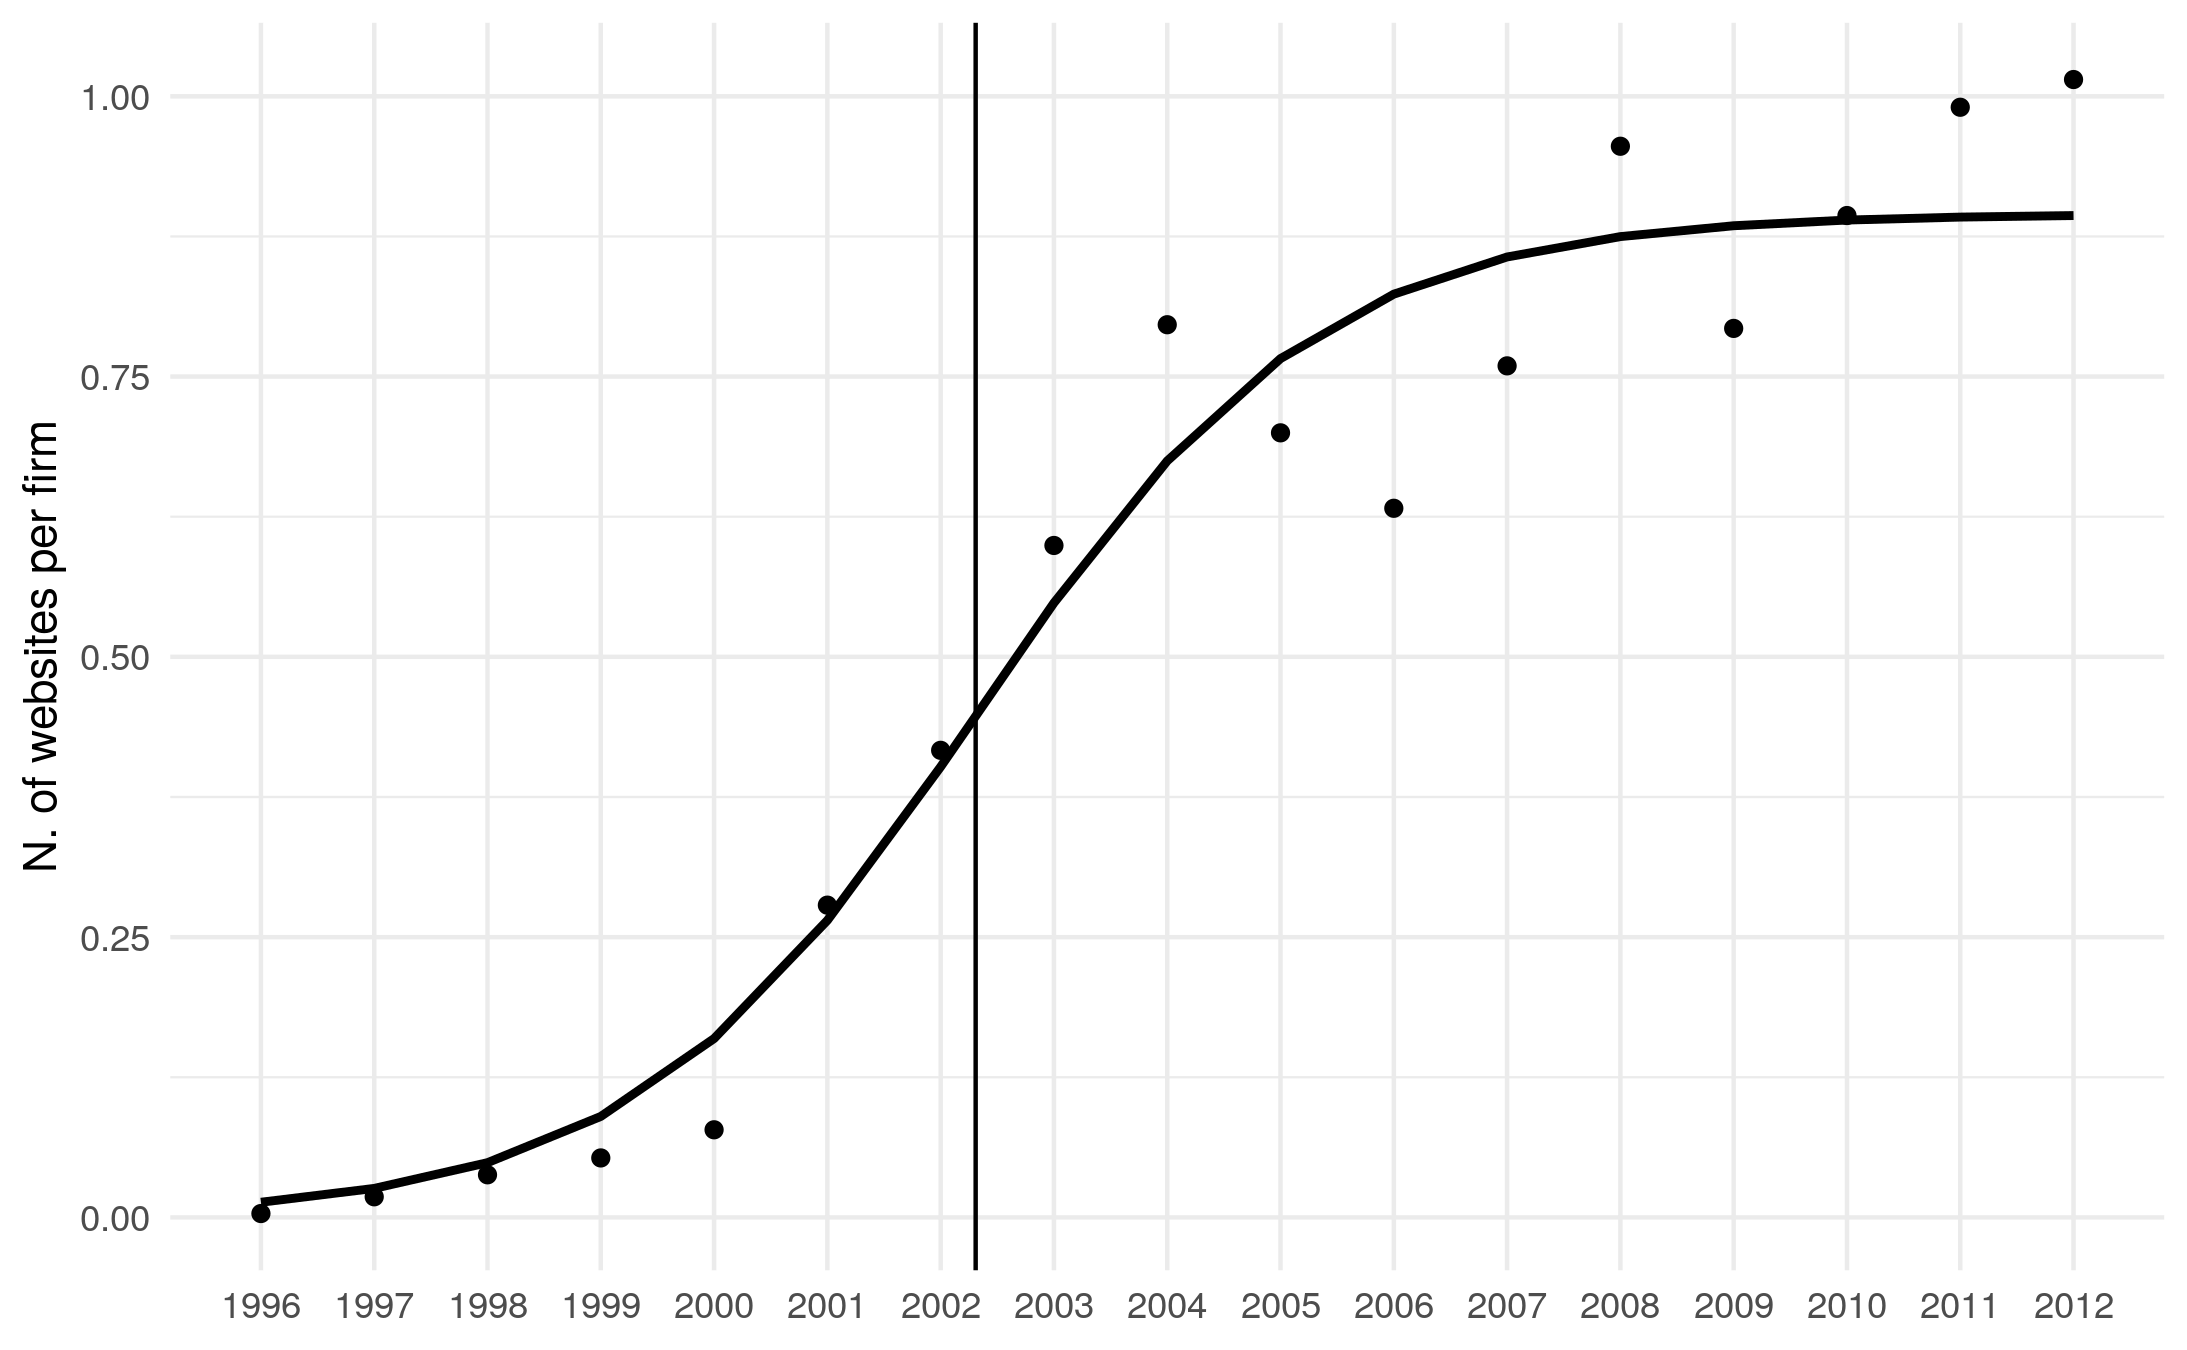
\includegraphics[width=1\textwidth,height=\textheight]{../../outputs/s/s_uk_per_firm_10.png}

}

\caption{\label{s_uk10}Cumulative adoption of the Web, UK; up to 10
postcodes per website}

\end{figure}%

\begin{figure}[H]

{\centering 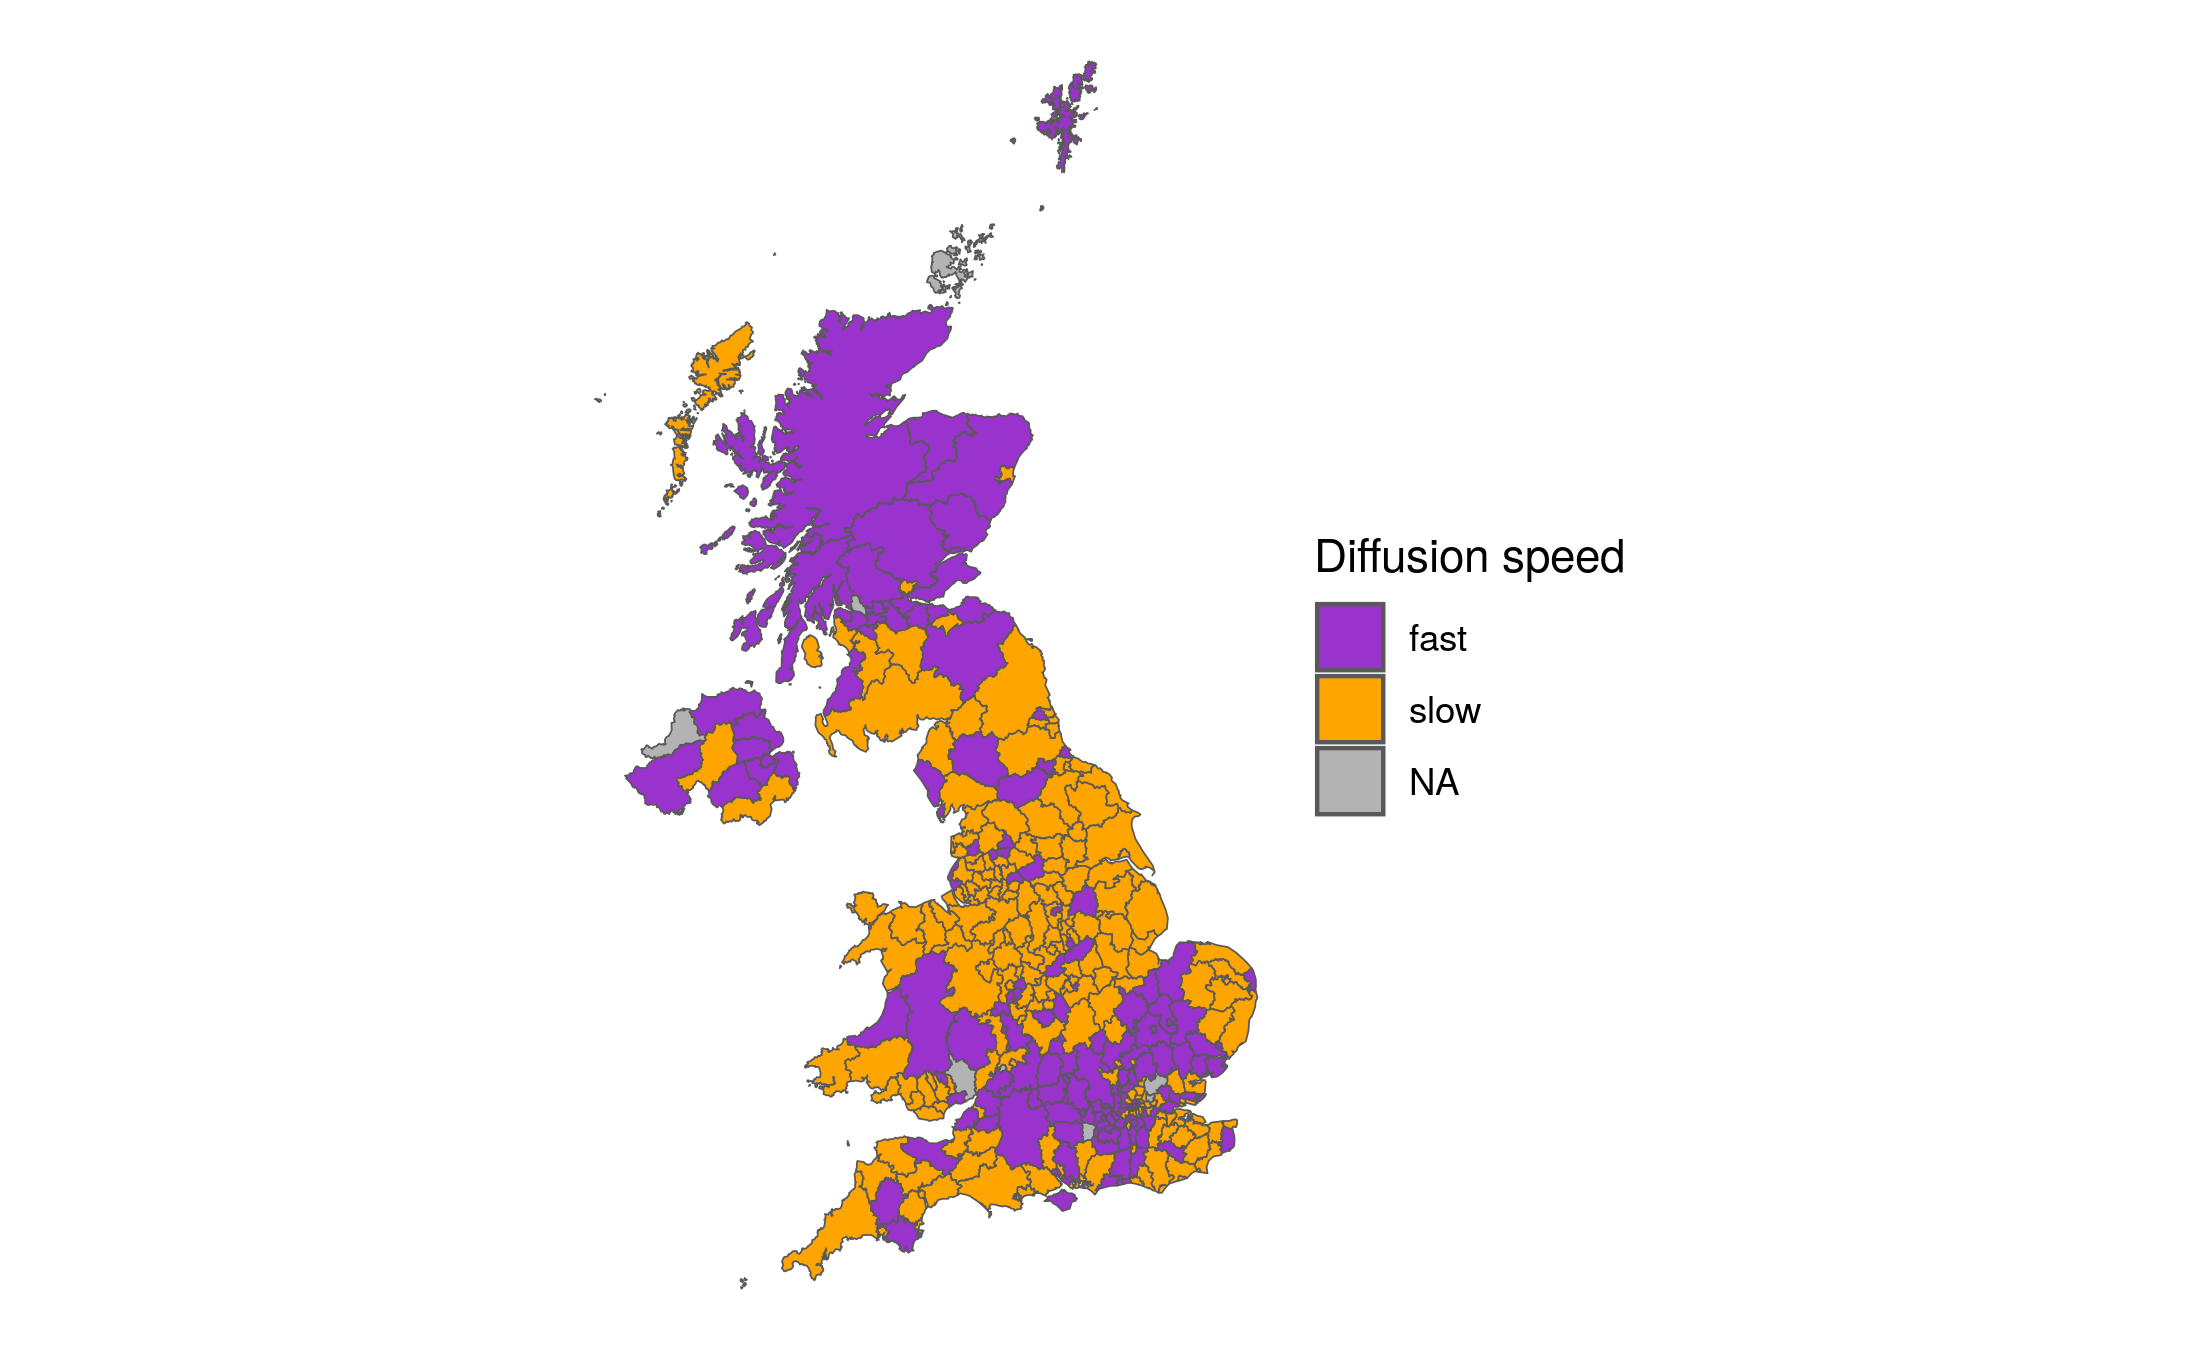
\includegraphics[width=1\textwidth,height=\textheight]{../../outputs/s/speed_map_10.png}

}

\caption{\label{s_map10}LAD Web diffusion speed, 1996-2012; up to 10
postcodes per website}

\end{figure}%

\begin{figure}[H]

{\centering 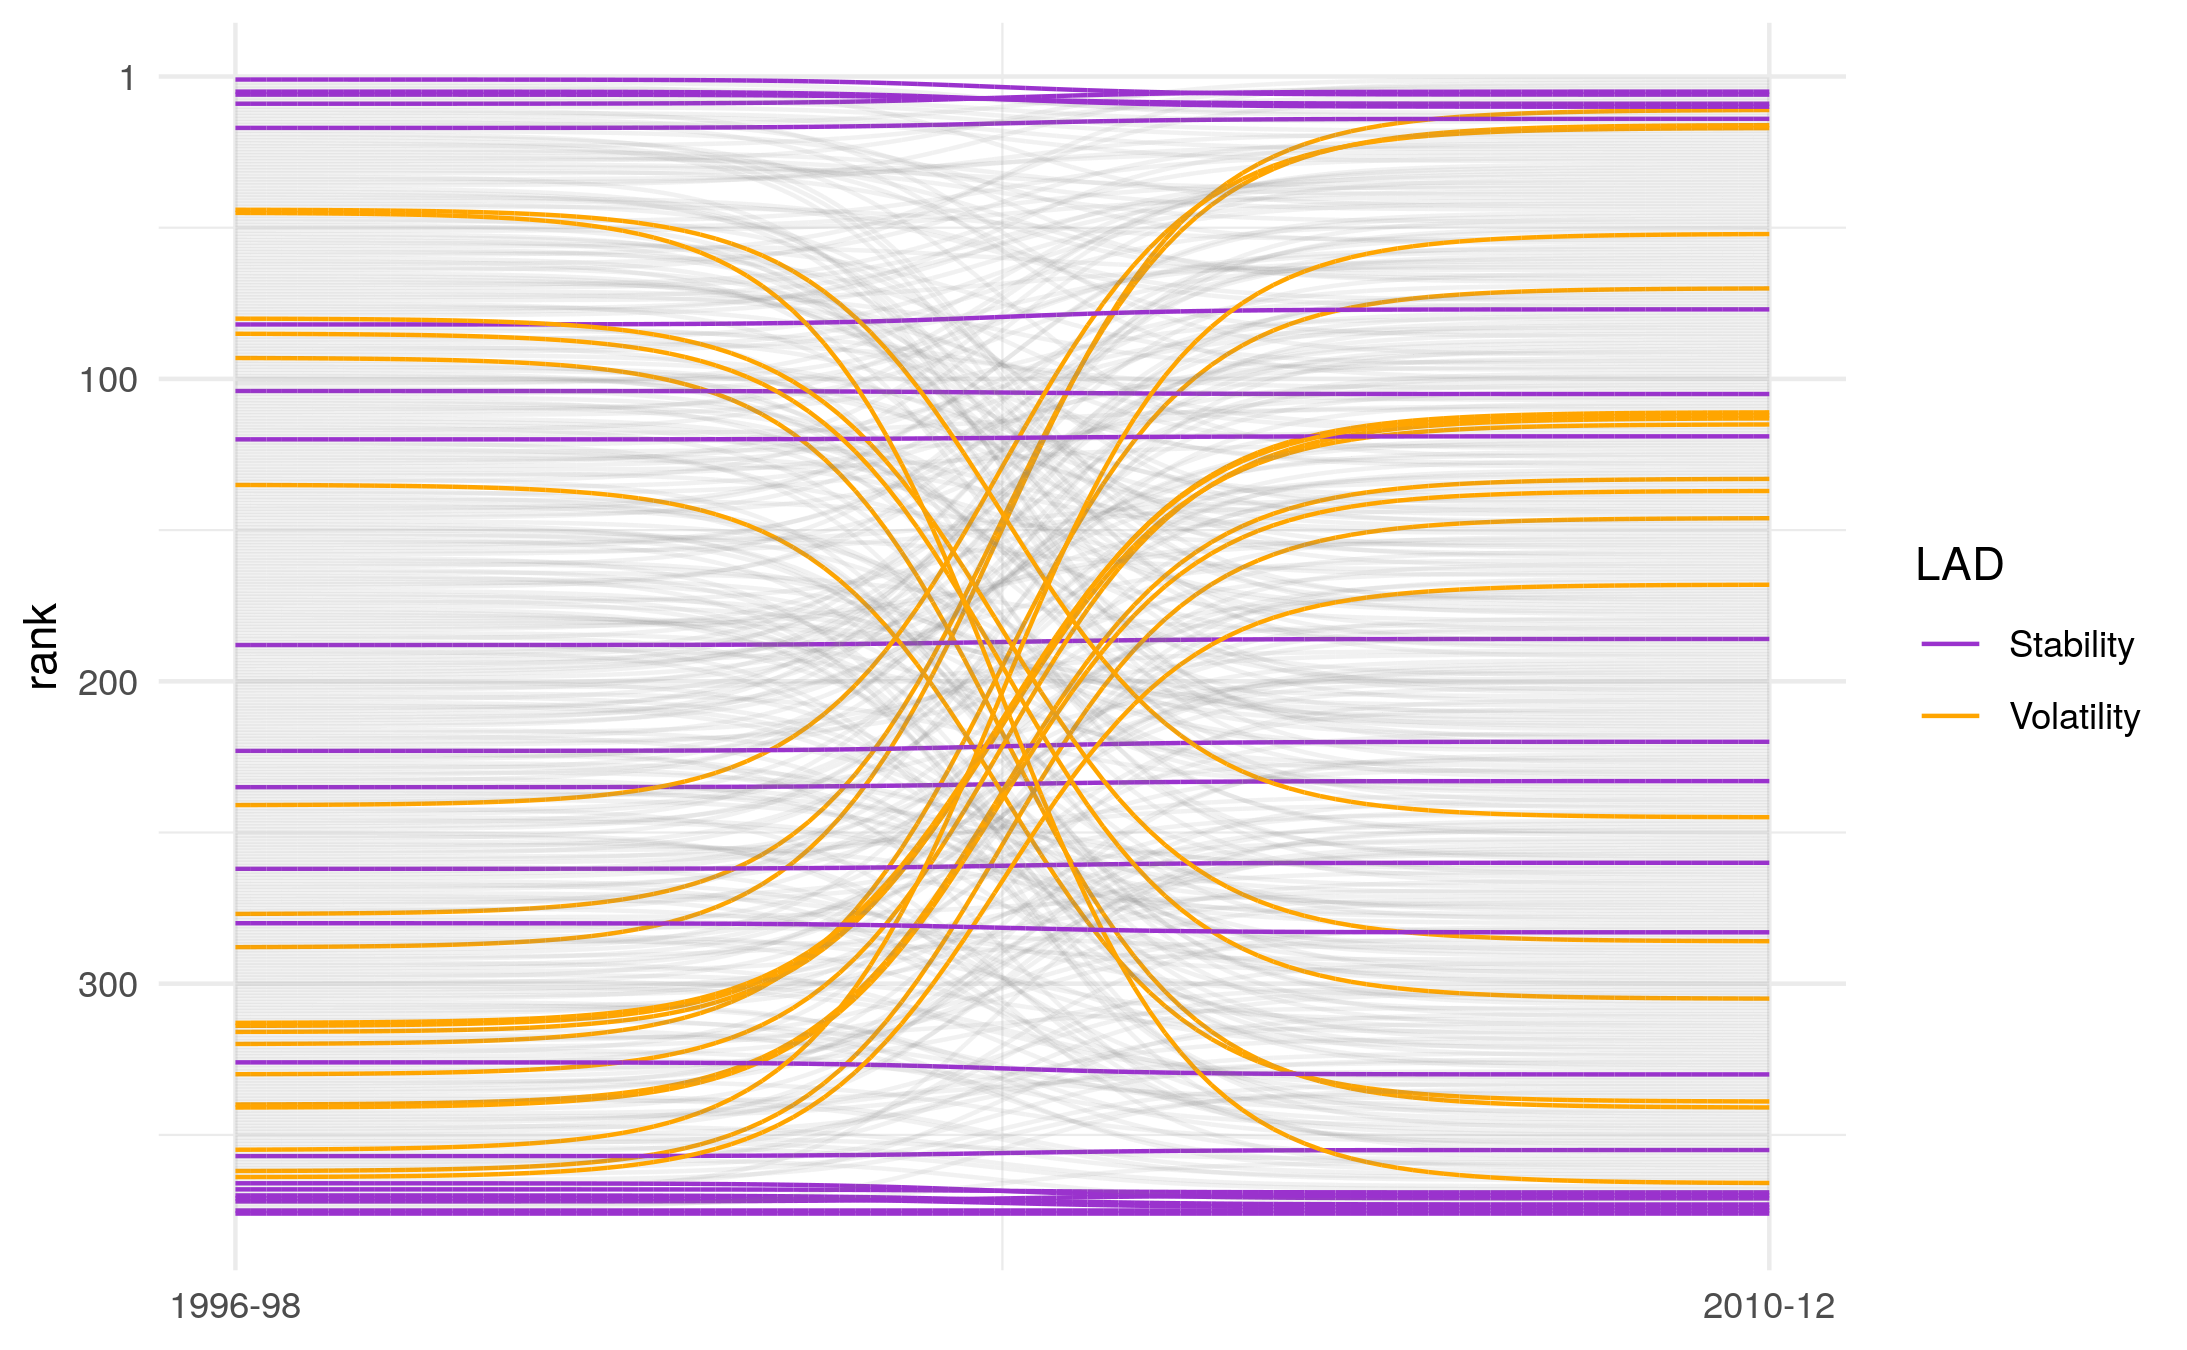
\includegraphics[width=1\textwidth,height=\textheight]{../../outputs/ranks/web_per_firm2000_2012_only0595_av_10.png}

}

\caption{\label{rank10}Dynamics of Web diffusion based on LAD rankings;
up to 10 postcodes per website}

\end{figure}%

\begin{figure}[H]

{\centering 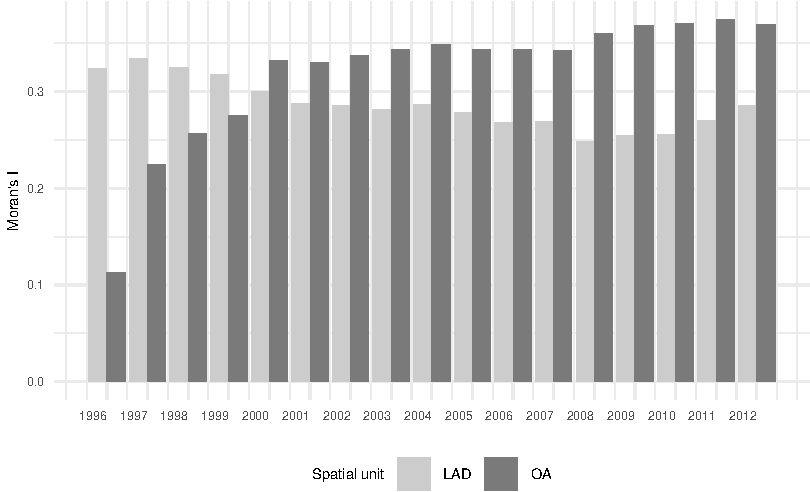
\includegraphics[width=1\textwidth,height=\textheight]{appendix_files/figure-pdf/morani10-1.pdf}

}

\caption{\label{morani10}Website density Moran's I; up to 10 postcodes
per website}

\end{figure}%

\begin{figure}[H]

{\centering 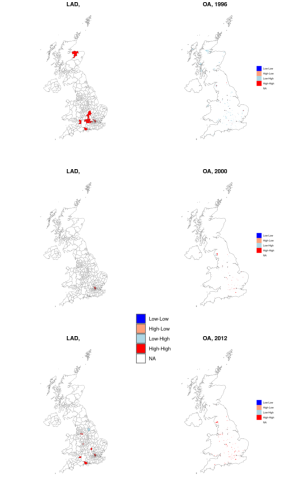
\includegraphics[width=1\textwidth,height=0.8\textheight]{appendix_files/figure-pdf/unnamed-chunk-4-1.pdf}

}

\caption{\label{lisa10}\centering Website density LISA maps; up to 10
postcodes per website}

\end{figure}%

\begin{figure}[H]

{\centering 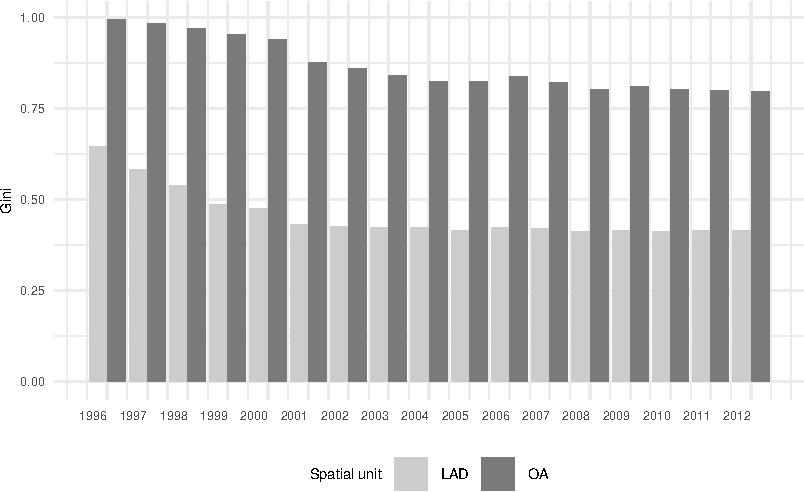
\includegraphics[width=1\textwidth,height=\textheight]{appendix_files/figure-pdf/gini10-1.pdf}

}

\caption{\label{gini10}Website density Gini coefficient; up to 10
postcodes per website}

\end{figure}%

\begin{figure}[H]

{\centering 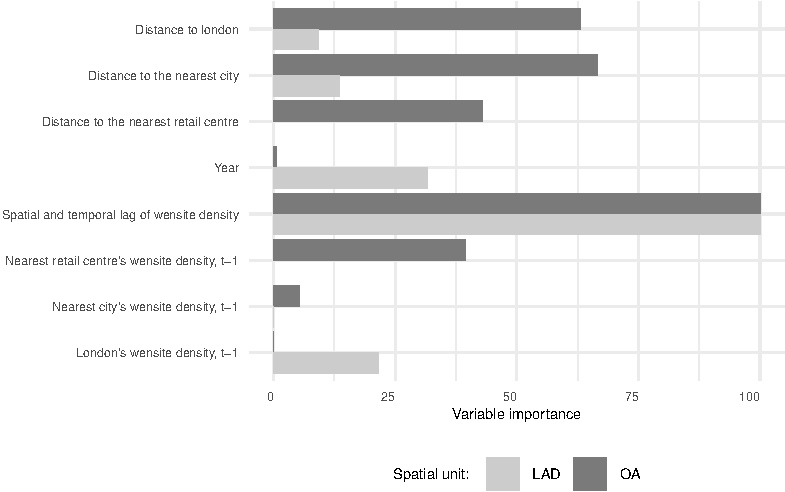
\includegraphics[width=1\textwidth,height=0.6\textheight]{appendix_files/figure-pdf/varimp10-1.pdf}

}

\caption{\label{var.imp10}Variable importance; up to 10 postcodes per
website}

\end{figure}%

\begin{longtable}[]{@{}
  >{\raggedright\arraybackslash}p{(\columnwidth - 10\tabcolsep) * \real{0.3186}}
  >{\raggedright\arraybackslash}p{(\columnwidth - 10\tabcolsep) * \real{0.2212}}
  >{\centering\arraybackslash}p{(\columnwidth - 10\tabcolsep) * \real{0.1416}}
  >{\centering\arraybackslash}p{(\columnwidth - 10\tabcolsep) * \real{0.1062}}
  >{\centering\arraybackslash}p{(\columnwidth - 10\tabcolsep) * \real{0.0619}}
  >{\centering\arraybackslash}p{(\columnwidth - 10\tabcolsep) * \real{0.1504}}@{}}
\caption{S-curve estiamtes for LAD\label{table.s.lads}}\tabularnewline
\toprule\noalign{}
\begin{minipage}[b]{\linewidth}\raggedright
LAD
\end{minipage} & \begin{minipage}[b]{\linewidth}\raggedright
Region
\end{minipage} & \begin{minipage}[b]{\linewidth}\centering
\(t_0\) estimate
\end{minipage} & \begin{minipage}[b]{\linewidth}\centering
Std. error
\end{minipage} & \begin{minipage}[b]{\linewidth}\centering
\(R^2\)
\end{minipage} & \begin{minipage}[b]{\linewidth}\centering
Diffusion speed
\end{minipage} \\
\midrule\noalign{}
\endfirsthead
\toprule\noalign{}
\begin{minipage}[b]{\linewidth}\raggedright
LAD
\end{minipage} & \begin{minipage}[b]{\linewidth}\raggedright
Region
\end{minipage} & \begin{minipage}[b]{\linewidth}\centering
\(t_0\) estimate
\end{minipage} & \begin{minipage}[b]{\linewidth}\centering
Std. error
\end{minipage} & \begin{minipage}[b]{\linewidth}\centering
\(R^2\)
\end{minipage} & \begin{minipage}[b]{\linewidth}\centering
Diffusion speed
\end{minipage} \\
\midrule\noalign{}
\endhead
\bottomrule\noalign{}
\endlastfoot
Horsham & South East & 2001.423 & 0.254 & 0.950 & fast \\
Fareham & South East & 2001.443 & 0.346 & 0.925 & fast \\
Kingston upon Thames & London & 2001.513 & 0.354 & 0.933 & fast \\
Kensington and Chelsea & London & 2001.581 & 0.341 & 0.943 & fast \\
Runnymede & South East & 2001.582 & 0.266 & 0.943 & fast \\
Bracknell Forest & South East & 2001.586 & 0.324 & 0.928 & fast \\
Elmbridge & South East & 2001.656 & 0.333 & 0.932 & fast \\
Reigate and Banstead & South East & 2001.665 & 0.253 & 0.964 & fast \\
South Cambridgeshire & East of England & 2001.680 & 0.433 & 0.905 &
fast \\
Walsall & West Midlands & 2001.715 & 0.413 & 0.901 & fast \\
Surrey Heath & South East & 2001.718 & 0.333 & 0.933 & fast \\
Woking & South East & 2001.759 & 0.292 & 0.951 & fast \\
South Norfolk & East of England & 2001.874 & 0.358 & 0.931 & fast \\
City of London & London & 2001.874 & 0.499 & 0.930 & fast \\
Wokingham & South East & 2001.891 & 0.287 & 0.958 & fast \\
Reading & South East & 2001.900 & 0.318 & 0.948 & fast \\
Sevenoaks & South East & 2001.904 & 0.407 & 0.926 & fast \\
Huntingdonshire & East of England & 2001.912 & 0.402 & 0.925 & fast \\
Pendle & North West & 2001.924 & 0.407 & 0.923 & fast \\
St Albans & East of England & 2001.933 & 0.396 & 0.927 & fast \\
Perth and Kinross & NA & 2001.943 & 0.228 & 0.970 & fast \\
Bromley & London & 2001.945 & 0.396 & 0.919 & fast \\
Rushmoor & South East & 2001.962 & 0.518 & 0.912 & fast \\
Powys & NA & 2001.969 & 0.278 & 0.963 & fast \\
Swindon & South West & 2001.996 & 0.390 & 0.916 & fast \\
Chelmsford & East of England & 2002.008 & 0.545 & 0.911 & fast \\
Crawley & South East & 2002.008 & 0.379 & 0.949 & fast \\
Dumfries and Galloway & NA & 2002.012 & 0.251 & 0.967 & fast \\
Inverclyde & NA & 2002.030 & 0.330 & 0.915 & fast \\
North Hertfordshire & East of England & 2002.031 & 0.475 & 0.920 &
fast \\
Moray & NA & 2002.050 & 0.358 & 0.947 & fast \\
Orkney Islands & NA & 2002.070 & 0.283 & 0.958 & fast \\
Fife & NA & 2002.070 & 0.363 & 0.945 & fast \\
Mole Valley & South East & 2002.071 & 0.460 & 0.925 & fast \\
Guildford & South East & 2002.113 & 0.413 & 0.941 & fast \\
Buckinghamshire & South East & 2002.114 & 0.390 & 0.942 & fast \\
Cotswold & South West & 2002.116 & 0.375 & 0.946 & fast \\
Shetland Islands & NA & 2002.120 & 0.332 & 0.949 & fast \\
South Oxfordshire & South East & 2002.146 & 0.367 & 0.950 & fast \\
Watford & East of England & 2002.157 & 0.451 & 0.929 & fast \\
Aberdeenshire & NA & 2002.168 & 0.416 & 0.931 & fast \\
Southampton & South East & 2002.189 & 0.472 & 0.922 & fast \\
Mid Suffolk & East of England & 2002.196 & 0.442 & 0.922 & fast \\
Eden & North West & 2002.196 & 0.334 & 0.949 & fast \\
South Lakeland & North West & 2002.197 & 0.238 & 0.974 & fast \\
Stoke-on-Trent & West Midlands & 2002.203 & 0.419 & 0.927 & fast \\
Babergh & East of England & 2002.209 & 0.449 & 0.927 & fast \\
Bexley & London & 2002.213 & 0.493 & 0.909 & fast \\
Torbay & South West & 2002.215 & 0.374 & 0.942 & fast \\
Brentwood & East of England & 2002.219 & 0.336 & 0.936 & fast \\
Ceredigion & NA & 2002.227 & 0.241 & 0.971 & fast \\
Spelthorne & South East & 2002.232 & 0.451 & 0.933 & fast \\
Bath and North East Somerset & South West & 2002.238 & 0.402 & 0.941 &
fast \\
Falkirk & NA & 2002.245 & 0.367 & 0.938 & fast \\
Broxtowe & East Midlands & 2002.258 & 0.435 & 0.932 & fast \\
East Hertfordshire & East of England & 2002.261 & 0.453 & 0.928 &
fast \\
Stirling & NA & 2002.268 & 0.251 & 0.975 & fast \\
Ealing & London & 2002.294 & 0.523 & 0.922 & fast \\
Mid Sussex & South East & 2002.295 & 0.453 & 0.936 & fast \\
Barrow-in-Furness & North West & 2002.303 & 0.284 & 0.959 & fast \\
West Oxfordshire & South East & 2002.322 & 0.467 & 0.929 & fast \\
Sutton & London & 2002.326 & 0.544 & 0.911 & fast \\
Portsmouth & South East & 2002.356 & 0.479 & 0.921 & fast \\
Great Yarmouth & East of England & 2002.369 & 0.265 & 0.968 & fast \\
East Hampshire & South East & 2002.370 & 0.474 & 0.931 & fast \\
Wyre Forest & West Midlands & 2002.376 & 0.561 & 0.916 & fast \\
Angus & NA & 2002.378 & 0.396 & 0.939 & fast \\
Argyll and Bute & NA & 2002.427 & 0.321 & 0.962 & fast \\
Scottish Borders & NA & 2002.428 & 0.298 & 0.962 & fast \\
East Suffolk & East of England & 2002.431 & 0.533 & 0.919 & fast \\
Blackpool & North West & 2002.443 & 0.294 & 0.962 & fast \\
Cherwell & South East & 2002.448 & 0.533 & 0.923 & fast \\
Wandsworth & London & 2002.449 & 0.570 & 0.921 & fast \\
Tendring & East of England & 2002.456 & 0.456 & 0.935 & fast \\
Westminster & London & 2002.459 & 0.437 & 0.952 & fast \\
Richmond upon Thames & London & 2002.462 & 0.389 & 0.956 & fast \\
Test Valley & South East & 2002.463 & 0.553 & 0.920 & fast \\
Isle of Wight & South East & 2002.478 & 0.377 & 0.953 & fast \\
Vale of White Horse & South East & 2002.496 & 0.408 & 0.949 & fast \\
Croydon & London & 2002.510 & 0.504 & 0.927 & fast \\
Hounslow & London & 2002.521 & 0.426 & 0.952 & fast \\
Copeland & North West & 2002.524 & 0.237 & 0.971 & fast \\
Wiltshire & South West & 2002.528 & 0.450 & 0.940 & fast \\
Gwynedd & NA & 2002.536 & 0.372 & 0.954 & fast \\
Hillingdon & London & 2002.560 & 0.470 & 0.940 & fast \\
Conwy & NA & 2002.564 & 0.372 & 0.954 & fast \\
Highland & NA & 2002.566 & 0.270 & 0.972 & fast \\
Basingstoke and Deane & South East & 2002.572 & 0.461 & 0.947 & fast \\
Harrow & London & 2002.587 & 0.509 & 0.936 & fast \\
West Berkshire & South East & 2002.595 & 0.696 & 0.902 & fast \\
North Lincolnshire & Yorkshire and The Humber & 2002.596 & 0.501 & 0.933
& fast \\
East Dunbartonshire & NA & 2002.598 & 0.528 & 0.925 & fast \\
Bradford & Yorkshire and The Humber & 2002.598 & 0.613 & 0.916 & fast \\
Waverley & South East & 2002.606 & 0.512 & 0.928 & fast \\
Stroud & South West & 2002.608 & 0.559 & 0.916 & fast \\
Herefordshire, County of & West Midlands & 2002.622 & 0.388 & 0.956 &
fast \\
North Norfolk & East of England & 2002.624 & 0.422 & 0.945 & fast \\
Nottingham & East Midlands & 2002.630 & 0.531 & 0.936 & fast \\
Castle Point & East of England & 2002.645 & 0.470 & 0.936 & fast \\
North Warwickshire & West Midlands & 2002.657 & 0.380 & 0.955 & fast \\
Gravesham & South East & 2002.680 & 0.473 & 0.933 & fast \\
Lancaster & North West & 2002.692 & 0.336 & 0.963 & fast \\
West Suffolk & East of England & 2002.699 & 0.536 & 0.930 & fast \\
Stafford & West Midlands & 2002.719 & 0.499 & 0.933 & fast \\
Tunbridge Wells & South East & 2002.720 & 0.401 & 0.958 & fast \\
Oxford & South East & 2002.723 & 0.583 & 0.934 & fast \\
East Lothian & NA & 2002.731 & 0.537 & 0.927 & fast \\
Redcar and Cleveland & North East & 2002.750 & 0.509 & 0.929 & fast \\
Tamworth & West Midlands & 2002.755 & 0.551 & 0.929 & fast \\
South Hams & South West & 2002.773 & 0.422 & 0.952 & fast \\
Allerdale & North West & 2002.784 & 0.376 & 0.958 & fast \\
Central Bedfordshire & East of England & 2002.825 & 0.620 & 0.921 &
fast \\
East Cambridgeshire & East of England & 2002.843 & 0.636 & 0.927 &
fast \\
Havant & South East & 2002.853 & 0.541 & 0.932 & fast \\
South Lanarkshire & NA & 2002.874 & 0.486 & 0.938 & fast \\
Stratford-on-Avon & West Midlands & 2002.879 & 0.470 & 0.945 & fast \\
Arun & South East & 2002.882 & 0.526 & 0.938 & fast \\
Fenland & East of England & 2002.891 & 0.632 & 0.918 & fast \\
Monmouthshire & NA & 2002.893 & 0.501 & 0.935 & fast \\
Denbighshire & NA & 2002.901 & 0.457 & 0.947 & fast \\
Southend-on-Sea & East of England & 2002.903 & 0.551 & 0.932 & fast \\
High Peak & East Midlands & 2002.903 & 0.488 & 0.946 & fast \\
Pembrokeshire & NA & 2002.905 & 0.387 & 0.958 & fast \\
Malvern Hills & West Midlands & 2002.907 & 0.524 & 0.940 & fast \\
Camden & London & 2002.915 & 0.599 & 0.941 & fast \\
North Devon & South West & 2002.926 & 0.426 & 0.950 & fast \\
Wyre & North West & 2002.927 & 0.553 & 0.927 & fast \\
Darlington & North East & 2002.933 & 0.615 & 0.929 & fast \\
Swale & South East & 2002.940 & 0.447 & 0.948 & fast \\
Welwyn Hatfield & East of England & 2002.951 & 0.628 & 0.922 & fast \\
Mid Devon & South West & 2002.960 & 0.485 & 0.946 & fast \\
Lewes & South East & 2002.964 & 0.507 & 0.945 & fast \\
Dorset & South West & 2002.968 & 0.407 & 0.958 & fast \\
Brighton and Hove & South East & 2002.976 & 0.578 & 0.934 & fast \\
Braintree & East of England & 2002.978 & 0.534 & 0.938 & fast \\
Epsom and Ewell & South East & 2002.979 & 0.746 & 0.908 & fast \\
Sefton & North West & 2002.980 & 0.616 & 0.928 & fast \\
Eastleigh & South East & 2002.992 & 0.595 & 0.929 & fast \\
Craven & Yorkshire and The Humber & 2002.993 & 0.379 & 0.965 & fast \\
Hammersmith and Fulham & London & 2002.997 & 0.585 & 0.944 & fast \\
Greenwich & London & 2003.014 & 0.571 & 0.930 & slow \\
Cheltenham & South West & 2003.025 & 0.602 & 0.937 & slow \\
Worcester & West Midlands & 2003.041 & 0.659 & 0.920 & slow \\
Tower Hamlets & London & 2003.043 & 0.660 & 0.926 & slow \\
New Forest & South East & 2003.046 & 0.554 & 0.941 & slow \\
East Renfrewshire & NA & 2003.046 & 0.739 & 0.900 & slow \\
Fylde & North West & 2003.056 & 0.501 & 0.946 & slow \\
Carmarthenshire & NA & 2003.067 & 0.390 & 0.958 & slow \\
West Lancashire & North West & 2003.076 & 0.547 & 0.937 & slow \\
Hastings & South East & 2003.086 & 0.685 & 0.911 & slow \\
Carlisle & North West & 2003.111 & 0.541 & 0.934 & slow \\
Wychavon & West Midlands & 2003.115 & 0.570 & 0.935 & slow \\
Isle of Anglesey & NA & 2003.144 & 0.403 & 0.960 & slow \\
Dudley & West Midlands & 2003.150 & 0.678 & 0.925 & slow \\
Ryedale & Yorkshire and The Humber & 2003.152 & 0.380 & 0.961 & slow \\
Rother & South East & 2003.162 & 0.366 & 0.966 & slow \\
Leicester & East Midlands & 2003.167 & 0.686 & 0.924 & slow \\
Breckland & East of England & 2003.182 & 0.567 & 0.938 & slow \\
Tandridge & South East & 2003.190 & 0.747 & 0.918 & slow \\
Shropshire & West Midlands & 2003.206 & 0.621 & 0.928 & slow \\
West Devon & South West & 2003.228 & 0.489 & 0.949 & slow \\
Milton Keynes & South East & 2003.231 & 0.700 & 0.929 & slow \\
Sandwell & West Midlands & 2003.234 & 0.760 & 0.916 & slow \\
Winchester & South East & 2003.234 & 0.443 & 0.956 & slow \\
Redditch & West Midlands & 2003.238 & 0.706 & 0.923 & slow \\
Rugby & West Midlands & 2003.265 & 0.709 & 0.922 & slow \\
North Somerset & South West & 2003.278 & 0.558 & 0.939 & slow \\
West Lindsey & East Midlands & 2003.285 & 0.674 & 0.924 & slow \\
Richmondshire & Yorkshire and The Humber & 2003.286 & 0.425 & 0.958 &
slow \\
Melton & East Midlands & 2003.292 & 0.534 & 0.946 & slow \\
Chichester & South East & 2003.295 & 0.582 & 0.942 & slow \\
Torridge & South West & 2003.301 & 0.532 & 0.942 & slow \\
Dundee City & NA & 2003.303 & 0.568 & 0.939 & slow \\
South Ayrshire & NA & 2003.303 & 0.626 & 0.931 & slow \\
East Devon & South West & 2003.308 & 0.492 & 0.947 & slow \\
Bolton & North West & 2003.323 & 0.774 & 0.913 & slow \\
Hertsmere & East of England & 2003.326 & 0.726 & 0.924 & slow \\
Bournemouth, Christchurch and Poole & South West & 2003.347 & 0.662 &
0.936 & slow \\
Maldon & East of England & 2003.349 & 0.495 & 0.951 & slow \\
Barnet & London & 2003.352 & 0.766 & 0.919 & slow \\
Brent & London & 2003.389 & 0.762 & 0.925 & slow \\
Midlothian & NA & 2003.413 & 0.732 & 0.921 & slow \\
Boston & East Midlands & 2003.416 & 0.593 & 0.933 & slow \\
Scarborough & Yorkshire and The Humber & 2003.421 & 0.431 & 0.963 &
slow \\
Kirklees & Yorkshire and The Humber & 2003.435 & 0.725 & 0.925 & slow \\
Tameside & North West & 2003.441 & 0.819 & 0.907 & slow \\
Newport & NA & 2003.449 & 0.635 & 0.930 & slow \\
Glasgow City & NA & 2003.451 & 0.759 & 0.922 & slow \\
Clackmannanshire & NA & 2003.454 & 0.585 & 0.936 & slow \\
Three Rivers & East of England & 2003.458 & 0.628 & 0.947 & slow \\
Harborough & East Midlands & 2003.488 & 0.549 & 0.950 & slow \\
Rochdale & North West & 2003.496 & 0.685 & 0.937 & slow \\
Tonbridge and Malling & South East & 2003.497 & 0.710 & 0.927 & slow \\
Somerset West and Taunton & South West & 2003.502 & 0.491 & 0.955 &
slow \\
Wrexham & NA & 2003.512 & 0.553 & 0.942 & slow \\
Worthing & South East & 2003.522 & 0.622 & 0.938 & slow \\
Tewkesbury & South West & 2003.540 & 0.580 & 0.946 & slow \\
City of Edinburgh & NA & 2003.541 & 0.685 & 0.941 & slow \\
Coventry & West Midlands & 2003.592 & 0.564 & 0.948 & slow \\
Northumberland & North East & 2003.607 & 0.508 & 0.954 & slow \\
Mid and East Antrim & NA & 2003.609 & 0.893 & 0.900 & slow \\
Wigan & North West & 2003.617 & 0.755 & 0.929 & slow \\
Lichfield & West Midlands & 2003.629 & 0.625 & 0.939 & slow \\
Ashford & South East & 2003.633 & 0.535 & 0.944 & slow \\
Cornwall & South West & 2003.638 & 0.443 & 0.963 & slow \\
Mendip & South West & 2003.652 & 0.505 & 0.955 & slow \\
Stevenage & East of England & 2003.665 & 0.525 & 0.958 & slow \\
Blaenau Gwent & NA & 2003.666 & 0.643 & 0.933 & slow \\
Lincoln & East Midlands & 2003.666 & 0.634 & 0.940 & slow \\
South Somerset & South West & 2003.676 & 0.553 & 0.948 & slow \\
Charnwood & East Midlands & 2003.677 & 0.699 & 0.934 & slow \\
North Ayrshire & NA & 2003.682 & 0.607 & 0.942 & slow \\
Folkestone and Hythe & South East & 2003.684 & 0.792 & 0.905 & slow \\
Eastbourne & South East & 2003.684 & 0.697 & 0.930 & slow \\
Blackburn with Darwen & North West & 2003.685 & 0.680 & 0.938 & slow \\
Dover & South East & 2003.699 & 0.574 & 0.948 & slow \\
Adur & South East & 2003.735 & 0.551 & 0.954 & slow \\
Haringey & London & 2003.739 & 0.667 & 0.943 & slow \\
Gosport & South East & 2003.751 & 0.600 & 0.934 & slow \\
Trafford & North West & 2003.752 & 0.640 & 0.949 & slow \\
Norwich & East of England & 2003.756 & 0.742 & 0.939 & slow \\
West Lothian & NA & 2003.758 & 0.652 & 0.943 & slow \\
North East Lincolnshire & Yorkshire and The Humber & 2003.811 & 0.858 &
0.920 & slow \\
Bristol, City of & South West & 2003.828 & 0.831 & 0.928 & slow \\
Rushcliffe & East Midlands & 2003.839 & 0.591 & 0.954 & slow \\
Hinckley and Bosworth & East Midlands & 2003.857 & 0.749 & 0.934 &
slow \\
Torfaen & NA & 2003.861 & 0.841 & 0.922 & slow \\
Swansea & NA & 2003.875 & 0.650 & 0.947 & slow \\
Wolverhampton & West Midlands & 2003.882 & 0.793 & 0.931 & slow \\
Kingston upon Hull, City of & Yorkshire and The Humber & 2003.885 &
0.757 & 0.936 & slow \\
Calderdale & Yorkshire and The Humber & 2003.889 & 0.714 & 0.939 &
slow \\
North Northamptonshire & East Midlands & 2003.902 & 0.746 & 0.935 &
slow \\
Stockton-on-Tees & North East & 2003.902 & 0.955 & 0.916 & slow \\
Wealden & South East & 2003.906 & 0.736 & 0.938 & slow \\
Thanet & South East & 2003.953 & 0.667 & 0.947 & slow \\
Broadland & East of England & 2003.962 & 0.727 & 0.938 & slow \\
West Northamptonshire & East Midlands & 2003.972 & 0.736 & 0.940 &
slow \\
North Kesteven & East Midlands & 2003.976 & 0.633 & 0.942 & slow \\
Neath Port Talbot & NA & 2003.981 & 0.767 & 0.933 & slow \\
Rhondda Cynon Taf & NA & 2003.991 & 0.769 & 0.925 & slow \\
Enfield & London & 2003.992 & 0.588 & 0.954 & slow \\
East Lindsey & East Midlands & 2004.010 & 0.577 & 0.952 & slow \\
Teignbridge & South West & 2004.015 & 0.681 & 0.941 & slow \\
York & Yorkshire and The Humber & 2004.025 & 0.739 & 0.944 & slow \\
Harlow & East of England & 2004.030 & 0.803 & 0.936 & slow \\
Vale of Glamorgan & NA & 2004.033 & 0.592 & 0.951 & slow \\
Newark and Sherwood & East Midlands & 2004.034 & 0.668 & 0.946 & slow \\
Merton & London & 2004.041 & 0.932 & 0.922 & slow \\
Hambleton & Yorkshire and The Humber & 2004.065 & 0.636 & 0.953 &
slow \\
Bedford & East of England & 2004.068 & 0.852 & 0.933 & slow \\
Stockport & North West & 2004.075 & 0.757 & 0.942 & slow \\
South Ribble & North West & 2004.126 & 0.674 & 0.948 & slow \\
Uttlesford & East of England & 2004.144 & 0.905 & 0.926 & slow \\
Rossendale & North West & 2004.160 & 0.976 & 0.923 & slow \\
Oldham & North West & 2004.162 & 0.801 & 0.938 & slow \\
Sheffield & Yorkshire and The Humber & 2004.189 & 0.770 & 0.944 &
slow \\
Ribble Valley & North West & 2004.204 & 0.718 & 0.945 & slow \\
Maidstone & South East & 2004.222 & 0.854 & 0.932 & slow \\
Cheshire West and Chester & North West & 2004.234 & 0.742 & 0.947 &
slow \\
Thurrock & East of England & 2004.241 & 0.841 & 0.924 & slow \\
Telford and Wrekin & West Midlands & 2004.241 & 1.024 & 0.917 & slow \\
Cardiff & NA & 2004.246 & 0.823 & 0.937 & slow \\
County Durham & North East & 2004.250 & 0.626 & 0.953 & slow \\
Plymouth & South West & 2004.252 & 0.785 & 0.934 & slow \\
Bridgend & NA & 2004.256 & 0.547 & 0.956 & slow \\
Rotherham & Yorkshire and The Humber & 2004.273 & 0.722 & 0.938 &
slow \\
Hyndburn & North West & 2004.298 & 0.881 & 0.932 & slow \\
Newcastle upon Tyne & North East & 2004.305 & 0.906 & 0.932 & slow \\
Wakefield & Yorkshire and The Humber & 2004.314 & 0.905 & 0.923 &
slow \\
Havering & London & 2004.345 & 0.822 & 0.938 & slow \\
South Kesteven & East Midlands & 2004.353 & 1.026 & 0.915 & slow \\
Canterbury & South East & 2004.354 & 0.602 & 0.960 & slow \\
Broxbourne & East of England & 2004.363 & 0.817 & 0.944 & slow \\
Peterborough & East of England & 2004.382 & 0.937 & 0.932 & slow \\
Redbridge & London & 2004.411 & 1.028 & 0.925 & slow \\
Bury & North West & 2004.431 & 0.735 & 0.953 & slow \\
Harrogate & Yorkshire and The Humber & 2004.433 & 0.971 & 0.927 &
slow \\
Birmingham & West Midlands & 2004.435 & 1.182 & 0.912 & slow \\
South Tyneside & North East & 2004.446 & 0.636 & 0.948 & slow \\
Chorley & North West & 2004.462 & 1.093 & 0.913 & slow \\
North East Derbyshire & East Midlands & 2004.483 & 0.703 & 0.953 &
slow \\
Lambeth & London & 2004.485 & 0.958 & 0.937 & slow \\
Doncaster & Yorkshire and The Humber & 2004.496 & 0.672 & 0.953 &
slow \\
South Gloucestershire & South West & 2004.499 & 0.881 & 0.937 & slow \\
Caerphilly & NA & 2004.499 & 0.819 & 0.938 & slow \\
East Staffordshire & West Midlands & 2004.501 & 1.132 & 0.910 & slow \\
North Tyneside & North East & 2004.509 & 0.864 & 0.933 & slow \\
South Holland & East Midlands & 2004.534 & 0.851 & 0.941 & slow \\
Gateshead & North East & 2004.535 & 0.869 & 0.934 & slow \\
St.~Helens & North West & 2004.542 & 1.097 & 0.923 & slow \\
Flintshire & NA & 2004.549 & 0.764 & 0.951 & slow \\
Selby & Yorkshire and The Humber & 2004.549 & 0.716 & 0.947 & slow \\
Belfast & NA & 2004.556 & 1.332 & 0.906 & slow \\
Sedgemoor & South West & 2004.613 & 0.540 & 0.966 & slow \\
Exeter & South West & 2004.617 & 0.964 & 0.936 & slow \\
South Derbyshire & East Midlands & 2004.629 & 0.934 & 0.938 & slow \\
Derbyshire Dales & East Midlands & 2004.668 & 0.648 & 0.963 & slow \\
East Riding of Yorkshire & Yorkshire and The Humber & 2004.683 & 0.728 &
0.955 & slow \\
Basildon & East of England & 2004.691 & 1.067 & 0.925 & slow \\
Barking and Dagenham & London & 2004.800 & 1.198 & 0.916 & slow \\
Causeway Coast and Glens & NA & 2004.834 & 1.024 & 0.928 & slow \\
North Lanarkshire & NA & 2004.839 & 0.878 & 0.945 & slow \\
Chesterfield & East Midlands & 2004.887 & 1.173 & 0.927 & slow \\
Newcastle-under-Lyme & West Midlands & 2004.933 & 1.172 & 0.925 &
slow \\
East Ayrshire & NA & 2004.934 & 1.280 & 0.903 & slow \\
Nuneaton and Bedworth & West Midlands & 2004.956 & 0.950 & 0.941 &
slow \\
Blaby & East Midlands & 2004.959 & 1.059 & 0.929 & slow \\
Leeds & Yorkshire and The Humber & 2004.979 & 0.836 & 0.956 & slow \\
Erewash & East Midlands & 2004.987 & 0.939 & 0.944 & slow \\
Bassetlaw & East Midlands & 2004.998 & 0.982 & 0.944 & slow \\
Hackney & London & 2005.026 & 1.157 & 0.934 & slow \\
Barnsley & Yorkshire and The Humber & 2005.055 & 0.912 & 0.942 & slow \\
Amber Valley & East Midlands & 2005.105 & 1.017 & 0.941 & slow \\
Colchester & East of England & 2005.144 & 1.250 & 0.927 & slow \\
Ashfield & East Midlands & 2005.176 & 1.073 & 0.942 & slow \\
Wirral & North West & 2005.184 & 1.084 & 0.939 & slow \\
Knowsley & North West & 2005.186 & 1.160 & 0.923 & slow \\
Windsor and Maidenhead & South East & 2005.195 & 1.746 & 0.902 & slow \\
Bromsgrove & West Midlands & 2005.494 & 1.144 & 0.941 & slow \\
Liverpool & North West & 2005.526 & 1.276 & 0.936 & slow \\
Staffordshire Moorlands & West Midlands & 2005.583 & 1.426 & 0.924 &
slow \\
Islington & London & 2005.970 & 1.223 & 0.955 & slow \\
Warrington & North West & 2006.015 & 1.387 & 0.942 & slow \\
Newham & London & 2006.078 & 1.908 & 0.907 & slow \\
Bolsover & East Midlands & 2006.188 & 1.143 & 0.957 & slow \\
Lisburn and Castlereagh & NA & 2006.193 & 1.970 & 0.903 & slow \\
Manchester & North West & 2006.449 & 1.434 & 0.950 & slow \\
Sunderland & North East & 2006.479 & 1.679 & 0.928 & slow \\
South Staffordshire & West Midlands & 2006.490 & 1.837 & 0.922 & slow \\
Rutland & East Midlands & 2006.529 & 0.986 & 0.967 & slow \\
Cannock Chase & West Midlands & 2006.700 & 2.231 & 0.917 & slow \\
Mansfield & East Midlands & 2006.889 & 1.579 & 0.946 & slow \\
Ards and North Down & NA & 2006.947 & 2.485 & 0.907 & slow \\
Halton & North West & 2007.069 & 0.932 & 0.967 & slow \\
Burnley & North West & 2007.372 & 2.286 & 0.919 & slow \\
Middlesbrough & North East & 2010.074 & 5.297 & 0.900 & slow \\
Isles of Scilly & South West & 2012.163 & 4.257 & 0.953 & slow \\
\end{longtable}

\begin{longtable}[]{@{}lrrrr@{}}
\caption{Regional differences; up to 10 postcodes per
website\label{table.regions.10}}\tabularnewline
\toprule\noalign{}
Region & \(R^2\) LAD & Rank LAD & \(R^2\) OA & Rank OA \\
\midrule\noalign{}
\endfirsthead
\toprule\noalign{}
Region & \(R^2\) LAD & Rank LAD & \(R^2\) OA & Rank OA \\
\midrule\noalign{}
\endhead
\bottomrule\noalign{}
\endlastfoot
Yorkshire and The Humber & 0.864 & 1 & 0.191 & 5 \\
West Midlands & 0.860 & 2 & 0.148 & 8 \\
South East & 0.848 & 3 & 0.171 & 7 \\
North West & 0.827 & 4 & 0.221 & 1 \\
London & 0.826 & 5 & 0.118 & 9 \\
South West & 0.801 & 6 & 0.194 & 4 \\
Wales & 0.746 & 7 & 0.114 & 11 \\
East Midlands & 0.732 & 8 & 0.117 & 10 \\
East of England & 0.731 & 9 & 0.178 & 6 \\
North East & 0.695 & 10 & 0.215 & 2 \\
Scotland & 0.588 & 11 & 0.052 & 12 \\
Nortern Ireland & 0.488 & 12 & 0.197 & 3 \\
\end{longtable}

\begin{longtable}[]{@{}llll@{}}
\caption{Model metrics for growth
model}\label{tbl-model-growth-metrics}\tabularnewline
\toprule\noalign{}
& \(RMSE\) & \(R^{2}\) & \(MAE\) \\
\midrule\noalign{}
\endfirsthead
\toprule\noalign{}
& \(RMSE\) & \(R^{2}\) & \(MAE\) \\
\midrule\noalign{}
\endhead
\bottomrule\noalign{}
\endlastfoot
Local Authorities & 0.286 & 0.506 & 0.223 \\
\end{longtable}

Table~\ref{tbl-model-growth-metrics} presents the results of a Random
Forest model that was trained based on Equation \ref{model.growth} using
all LAD data points. In essence, this is a model similar to the one
estimated based on Equation 3 and presented in Table 2, with the main
difference being the dependent variable which is the year growth rate of
website density for each LAD. To avoid cases with LAD have no websites,
\(t \in [2000, 2012]\). The high predictive capability of the model
reflects the robustness of the modelling approach.

\begin{align} \label{model.growth}
Website\,Density\,Growth_{t} \sim Distance\,London +
Website\,density\,London_{t-1} +\notag\\
Distance\,Nearest\,City +
Website\,density\,Nearest\,City_{t-1} +\notag\\
Distance\,Nearest\,Retail_{i} +
Website\,density\,Nearest\,Retail_{t-1} +\notag\\
W*\, Website\,density_{t-1} +\notag\\ 
year_{t}
\end{align}




\end{document}
